\documentclass[11pt,a4paper]{article}

% ============================================
% PACKAGES
% ============================================
\usepackage[margin=1in]{geometry}
\usepackage{amsmath}
\usepackage{amssymb}
\usepackage{amsthm}
\usepackage{tikz}
\usepackage{pgfplots}
\pgfplotsset{compat=1.17}
\usepackage[most]{tcolorbox}
\usepackage{listings}
\usepackage{hyperref}
\usepackage{xcolor}
\usepackage{enumitem}
\usepackage{multicol}
\usepackage{array}

% TikZ libraries
\usetikzlibrary{arrows.meta, positioning, shapes.geometric, patterns}

% Hyperref setup
\hypersetup{
    colorlinks=true,
    linkcolor=blue,
    urlcolor=cyan,
    citecolor=green
}

% ============================================
% THEOREM ENVIRONMENTS
% ============================================
\theoremstyle{definition}
\newtheorem{definition}{Definition}[section]
\newtheorem{example}{Example}[section]
\newtheorem{remark}{Remark}[section]

\theoremstyle{plain}
\newtheorem{theorem}{Theorem}[section]
\newtheorem{lemma}{Lemma}[section]

% ============================================
% CUSTOM BOXES
% ============================================

% Definition box (blue)
\newtcolorbox{defbox}[1]{
    colback=blue!5!white,
    colframe=blue!75!black,
    fonttitle=\bfseries,
    title=#1
}

% Theorem box (green)
\newtcolorbox{thmbox}[1]{
    colback=green!5!white,
    colframe=green!75!black,
    fonttitle=\bfseries,
    title=#1
}

% Warning box (red/orange)
\newtcolorbox{warnbox}[1]{
    colback=orange!5!white,
    colframe=orange!75!black,
    fonttitle=\bfseries,
    title=#1
}

% Exam tips box (yellow)
\newtcolorbox{exambox}[1]{
    colback=yellow!10!white,
    colframe=yellow!75!black,
    fonttitle=\bfseries,
    title=#1
}

% Example box
\newtcolorbox{examplebox}[1]{
    colback=gray!5!white,
    colframe=gray!75!black,
    fonttitle=\bfseries,
    title=#1
}

% ============================================
% TITLE AND DOCUMENT INFO
% ============================================
\title{\textbf{STA 351: Probability Models and Inference}\\
\Large Module 1: Foundations of Multiple Random Variables\\
Joint Distributions}
\author{Exam-Focused Study Notes}
\date{\today}

% ============================================
% CUSTOM COMMANDS
% ============================================
\newcommand{\E}{\mathbb{E}}
\newcommand{\Var}{\text{Var}}
\newcommand{\Cov}{\text{Cov}}
\newcommand{\Corr}{\text{Corr}}
\newcommand{\R}{\mathbb{R}}
\newcommand{\N}{\mathbb{N}}

% ============================================
% DOCUMENT
% ============================================
\begin{document}

\maketitle
\tableofcontents
\newpage

% ============================================
% INTRODUCTION
% ============================================
\section*{Introduction}
\addcontentsline{toc}{section}{Introduction}

This document provides a comprehensive, exam-focused review of Module 1 for STA 351: Probability Models and Inference. The material covers joint distributions of multiple random variables, including both discrete and continuous cases.

\begin{exambox}{Study Strategy}
\begin{itemize}
    \item \textbf{Focus on understanding} the intuition before memorizing formulas
    \item \textbf{Practice problems} are your best preparation
    \item \textbf{Pay attention to warnings} about common mistakes
    \item \textbf{Know the difference} between discrete and continuous cases
    \item \textbf{Memorize key formulas} highlighted in boxes
\end{itemize}
\end{exambox}

% ============================================
% SECTION 1.1: JOINT DISTRIBUTIONS
% ============================================
\section{Joint Distributions}

\subsection{Joint PMF (Discrete Case)}

\begin{defbox}{Joint Probability Mass Function (PMF)}
For discrete random variables $X$ and $Y$, the \textbf{joint PMF} is defined as:
\[
p_{X,Y}(x, y) = P(X = x, Y = y)
\]

\textbf{Intuition:} Think of the joint PMF as a 2D probability table where each cell $(x,y)$ tells you the probability that $X$ takes value $x$ AND $Y$ takes value $y$ simultaneously.
\end{defbox}

\textbf{Properties:}
\begin{enumerate}
    \item \textbf{Non-negativity:} $p_{X,Y}(x, y) \geq 0$ for all $x, y$
    \item \textbf{Normalization:} $\displaystyle\sum_x \sum_y p_{X,Y}(x, y) = 1$ (sum over all possible values)
\end{enumerate}

\textbf{Visual Representation:}

\begin{center}
\begin{tabular}{c|c|c|c|c}
    \diagbox{$X$}{$Y$} & $y_1$ & $y_2$ & $y_3$ & $p_X(x)$ \\
    \hline
    $x_1$ & $p_{X,Y}(x_1,y_1)$ & $p_{X,Y}(x_1,y_2)$ & $p_{X,Y}(x_1,y_3)$ & $\sum_y p_{X,Y}(x_1,y)$ \\
    $x_2$ & $p_{X,Y}(x_2,y_1)$ & $p_{X,Y}(x_2,y_2)$ & $p_{X,Y}(x_2,y_3)$ & $\sum_y p_{X,Y}(x_2,y)$ \\
    \hline
    $p_Y(y)$ & $\sum_x p_{X,Y}(x,y_1)$ & $\sum_x p_{X,Y}(x,y_2)$ & $\sum_x p_{X,Y}(x,y_3)$ & 1
\end{tabular}
\end{center}

\begin{examplebox}{Example 1.1: Joint PMF}
\textbf{Problem:} Two fair dice are rolled. Let $X$ be the value on the first die and $Y$ be the value on the second die. Find $p_{X,Y}(3, 4)$.

\textbf{Solution:}
\begin{align*}
p_{X,Y}(3, 4) &= P(X = 3, Y = 4) \\
&= P(\text{first die shows 3 AND second die shows 4}) \\
&= \frac{1}{6} \times \frac{1}{6} = \frac{1}{36}
\end{align*}

Since the dice are independent, the joint probability is the product of individual probabilities.
\end{examplebox}

\subsection{Joint PDF (Continuous Case)}

\begin{defbox}{Joint Probability Density Function (PDF)}
For continuous random variables $X$ and $Y$, the \textbf{joint PDF} $f_{X,Y}(x, y)$ satisfies:
\[
P((X,Y) \in A) = \iint_A f_{X,Y}(x, y)\, dx\, dy
\]

\textbf{Geometric Interpretation:} The probability is the \textbf{volume under the surface} $z = f_{X,Y}(x, y)$ over the region $A$ in the $xy$-plane.
\end{defbox}

\textbf{Properties:}
\begin{enumerate}
    \item \textbf{Non-negativity:} $f_{X,Y}(x, y) \geq 0$ for all $x, y$
    \item \textbf{Normalization:} $\displaystyle\int_{-\infty}^{\infty} \int_{-\infty}^{\infty} f_{X,Y}(x, y)\, dx\, dy = 1$
\end{enumerate}

\textbf{Visualization:}

\begin{center}
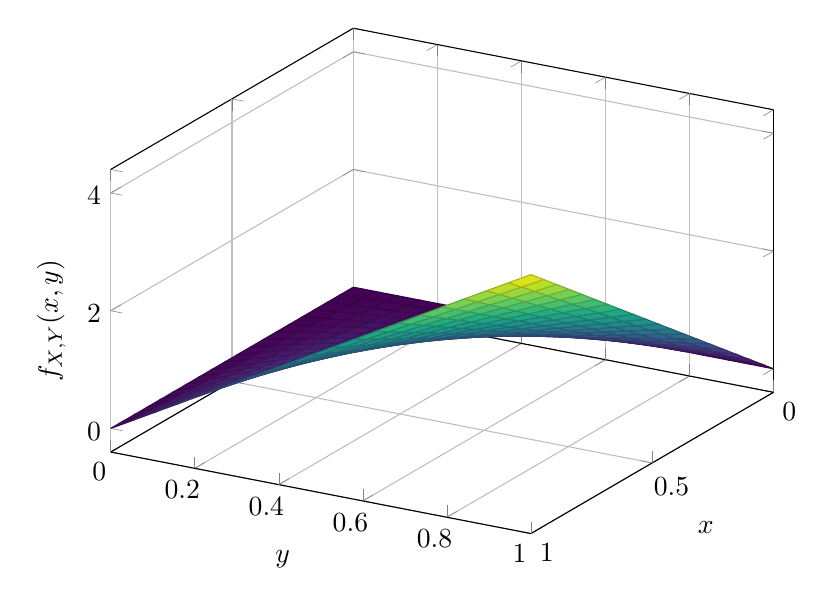
\begin{tikzpicture}
\begin{axis}[
    width=10cm,
    height=8cm,
    xlabel=$x$,
    ylabel=$y$,
    zlabel={$f_{X,Y}(x,y)$},
    view={120}{30},
    grid=major,
    colormap/viridis,
]
\addplot3[
    surf,
    domain=0:1,
    domain y=0:1,
    samples=20,
] {4*x*y};
\end{axis}
\end{tikzpicture}
\end{center}

\begin{examplebox}{Example 1.2: Uniform Distribution over a Region}
\textbf{Problem:} Let $(X,Y)$ be uniformly distributed over the triangular region $D = \{(x,y) : 0 \leq x \leq 1, 0 \leq y \leq x\}$. Find the joint PDF.

\textbf{Solution:}

Step 1: Find the area of the region $D$:
\[
\text{Area}(D) = \int_0^1 \int_0^x dy\, dx = \int_0^1 x\, dx = \frac{1}{2}
\]

Step 2: For a uniform distribution, the PDF is constant over $D$:
\[
f_{X,Y}(x, y) = \begin{cases}
\frac{1}{\text{Area}(D)} = 2 & \text{if } (x,y) \in D \\
0 & \text{otherwise}
\end{cases}
\]

Step 3: Verify normalization:
\[
\int_0^1 \int_0^x 2\, dy\, dx = 2 \cdot \frac{1}{2} = 1 \quad \checkmark
\]
\end{examplebox}

\subsection{Joint CDF and Properties}

\begin{defbox}{Joint Cumulative Distribution Function (CDF)}
The \textbf{joint CDF} is defined as:
\[
F_{X,Y}(x, y) = P(X \leq x, Y \leq y)
\]

\textbf{For discrete:} $F_{X,Y}(x, y) = \sum_{s \leq x} \sum_{t \leq y} p_{X,Y}(s, t)$

\textbf{For continuous:} $F_{X,Y}(x, y) = \int_{-\infty}^x \int_{-\infty}^y f_{X,Y}(s, t)\, dt\, ds$
\end{defbox}

\textbf{Key Properties:}
\begin{enumerate}
    \item \textbf{Limits at boundaries:}
    \begin{itemize}
        \item $F_{X,Y}(-\infty, y) = 0$
        \item $F_{X,Y}(x, -\infty) = 0$
        \item $F_{X,Y}(\infty, \infty) = 1$
    \end{itemize}
    \item \textbf{Non-decreasing:} $F_{X,Y}$ is non-decreasing in each argument
    \item \textbf{Right-continuity:} $F_{X,Y}$ is right-continuous in each argument
\end{enumerate}

\textbf{Rectangle Formula:}
\[
P(a < X \leq b, c < Y \leq d) = F_{X,Y}(b,d) - F_{X,Y}(a,d) - F_{X,Y}(b,c) + F_{X,Y}(a,c)
\]

\begin{center}
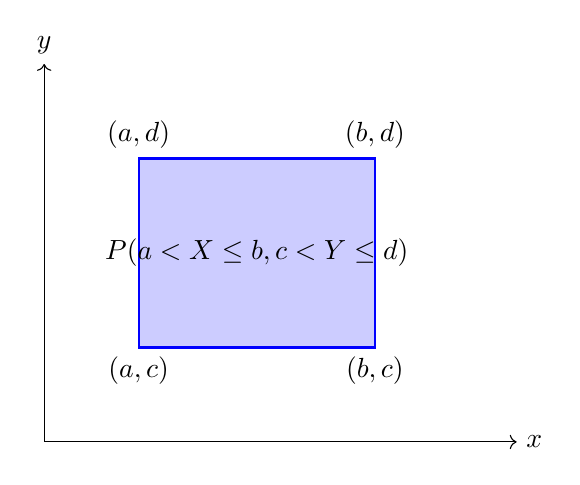
\begin{tikzpicture}[scale=1.2]
    % Draw axes
    \draw[->] (0,0) -- (5,0) node[right] {$x$};
    \draw[->] (0,0) -- (0,4) node[above] {$y$};
    
    % Draw rectangle
    \draw[thick, blue] (1,1) rectangle (3.5,3);
    
    % Label points
    \node[below] at (1,1) {$(a,c)$};
    \node[below] at (3.5,1) {$(b,c)$};
    \node[above] at (1,3) {$(a,d)$};
    \node[above] at (3.5,3) {$(b,d)$};
    
    % Add shading
    \fill[blue, opacity=0.2] (1,1) rectangle (3.5,3);
    
    % Add labels
    \node at (2.25,2) {$P(a < X \leq b, c < Y \leq d)$};
\end{tikzpicture}
\end{center}

\subsection{Independence of Random Variables}

\begin{defbox}{Independence}
Random variables $X$ and $Y$ are \textbf{independent} if and only if:
\[
f_{X,Y}(x, y) = f_X(x) \cdot f_Y(y) \quad \text{for all } x, y
\]

Or equivalently: $F_{X,Y}(x, y) = F_X(x) \cdot F_Y(y)$ for all $x, y$.

\textbf{Intuition:} Knowing the value of $X$ tells you \textbf{nothing} about the value of $Y$.
\end{defbox}

\textbf{Test for Independence:}
\begin{enumerate}
    \item Find the marginal distributions $f_X(x)$ and $f_Y(y)$
    \item Check if $f_{X,Y}(x, y) = f_X(x) \cdot f_Y(y)$ for \textbf{all} $(x,y)$
    \item If the equation holds for all $(x,y)$, then $X$ and $Y$ are independent
    \item If it fails for even \textbf{one} pair $(x,y)$, they are \textbf{not} independent
\end{enumerate}

\begin{warnbox}{Common Mistake: Independence Test}
\textbf{WARNING:} Checking only that $\E[XY] = \E[X]\E[Y]$ is \textbf{NOT sufficient} to prove independence!

This condition only shows that $X$ and $Y$ are \textbf{uncorrelated}, which is a weaker condition than independence.

\textbf{Remember:}
\begin{center}
Independent $\Rightarrow$ Uncorrelated

Uncorrelated $\not\Rightarrow$ Independent
\end{center}

You must verify the factorization of the joint distribution!
\end{warnbox}

\begin{examplebox}{Example 1.3: Testing Independence}
\textbf{Problem:} Consider the following joint PMF for $X$ and $Y$:

\begin{center}
\begin{tabular}{c|cc|c}
    $X \backslash Y$ & 0 & 1 & $p_X(x)$ \\
    \hline
    0 & 0.2 & 0.3 & 0.5 \\
    1 & 0.3 & 0.2 & 0.5 \\
    \hline
    $p_Y(y)$ & 0.5 & 0.5 & 1
\end{tabular}
\end{center}

Are $X$ and $Y$ independent?

\textbf{Solution:}

Check if $p_{X,Y}(x,y) = p_X(x) \cdot p_Y(y)$ for all $(x,y)$:

For $(0,0)$: $p_{X,Y}(0,0) = 0.2$ but $p_X(0) \cdot p_Y(0) = 0.5 \times 0.5 = 0.25$

Since $0.2 \neq 0.25$, the factorization fails.

\textbf{Conclusion:} $X$ and $Y$ are \textbf{NOT} independent.
\end{examplebox}

% ============================================
% SECTION 1.2: MARGINAL DISTRIBUTIONS
% ============================================
\section{Marginal Distributions}

\subsection{Finding Marginal PMF/PDF}

\begin{defbox}{Marginal Distributions}
The \textbf{marginal distribution} of $X$ is obtained by "summing out" (discrete) or "integrating out" (continuous) the other variable $Y$.

\textbf{Discrete Case:}
\[
p_X(x) = \sum_y p_{X,Y}(x, y)
\]
\[
p_Y(y) = \sum_x p_{X,Y}(x, y)
\]

\textbf{Continuous Case:}
\[
f_X(x) = \int_{-\infty}^{\infty} f_{X,Y}(x, y)\, dy
\]
\[
f_Y(y) = \int_{-\infty}^{\infty} f_{X,Y}(x, y)\, dx
\]

\textbf{Intuition:} Marginals are the "shadows" or "projections" of the joint distribution onto each axis.
\end{defbox}

\textbf{Visual Interpretation:}

\begin{center}
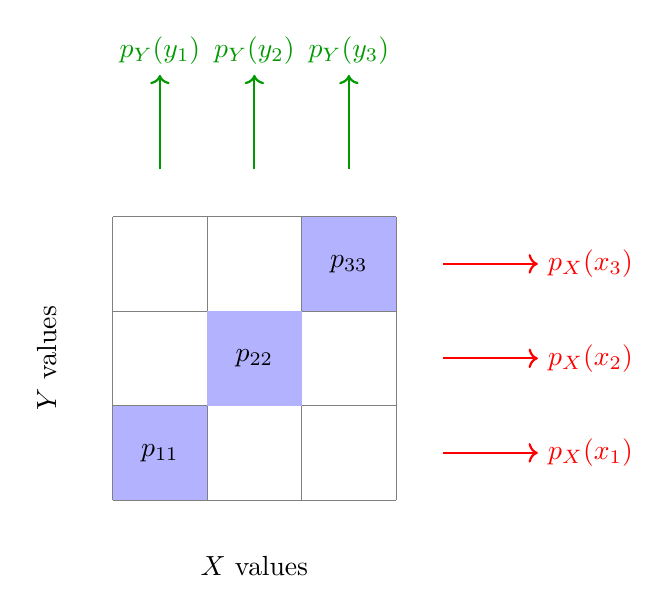
\begin{tikzpicture}[scale=1.2]
    % Main joint distribution table
    \draw[step=1cm, gray, very thin] (0,0) grid (3,3);
    \fill[blue!30] (0,0) rectangle (1,1);
    \fill[blue!30] (1,1) rectangle (2,2);
    \fill[blue!30] (2,2) rectangle (3,3);
    
    % Labels for the grid
    \node at (0.5,0.5) {$p_{11}$};
    \node at (1.5,1.5) {$p_{22}$};
    \node at (2.5,2.5) {$p_{33}$};
    
    % Marginal sums on sides
    \draw[thick, red, ->] (3.5,0.5) -- (4.5,0.5) node[right] {$p_X(x_1)$};
    \draw[thick, red, ->] (3.5,1.5) -- (4.5,1.5) node[right] {$p_X(x_2)$};
    \draw[thick, red, ->] (3.5,2.5) -- (4.5,2.5) node[right] {$p_X(x_3)$};
    
    \draw[thick, green!60!black, ->] (0.5,3.5) -- (0.5,4.5) node[above] {$p_Y(y_1)$};
    \draw[thick, green!60!black, ->] (1.5,3.5) -- (1.5,4.5) node[above] {$p_Y(y_2)$};
    \draw[thick, green!60!black, ->] (2.5,3.5) -- (2.5,4.5) node[above] {$p_Y(y_3)$};
    
    % Axis labels
    \node at (1.5,-0.7) {$X$ values};
    \node[rotate=90] at (-0.7,1.5) {$Y$ values};
\end{tikzpicture}
\end{center}

\begin{examplebox}{Example 1.4: Finding Marginals (Discrete)}
\textbf{Problem:} Given the joint PMF:

\begin{center}
\begin{tabular}{c|ccc}
    $X \backslash Y$ & 1 & 2 & 3 \\
    \hline
    1 & 0.1 & 0.1 & 0.2 \\
    2 & 0.2 & 0.3 & 0.1 \\
\end{tabular}
\end{center}

Find the marginal PMFs of $X$ and $Y$.

\textbf{Solution:}

For $X$:
\begin{align*}
p_X(1) &= 0.1 + 0.1 + 0.2 = 0.4 \\
p_X(2) &= 0.2 + 0.3 + 0.1 = 0.6
\end{align*}

For $Y$:
\begin{align*}
p_Y(1) &= 0.1 + 0.2 = 0.3 \\
p_Y(2) &= 0.1 + 0.3 = 0.4 \\
p_Y(3) &= 0.2 + 0.1 = 0.3
\end{align*}
\end{examplebox}

\begin{examplebox}{Example 1.5: Finding Marginals (Continuous)}
\textbf{Problem:} Let $f_{X,Y}(x,y) = 2$ for $0 \leq y \leq x \leq 1$, and $0$ otherwise. Find $f_X(x)$ and $f_Y(y)$.

\textbf{Solution:}

For $f_X(x)$ where $0 \leq x \leq 1$:
\[
f_X(x) = \int_{-\infty}^{\infty} f_{X,Y}(x,y)\, dy = \int_0^x 2\, dy = 2x
\]

For $f_Y(y)$ where $0 \leq y \leq 1$:
\[
f_Y(y) = \int_{-\infty}^{\infty} f_{X,Y}(x,y)\, dx = \int_y^1 2\, dx = 2(1-y)
\]
\end{examplebox}

\subsection{Relationship Between Joint and Marginal}

\begin{exambox}{Key Insight About Joint and Marginal Distributions}
\textbf{Important Exam Concept:}

\begin{enumerate}
    \item You can \textbf{ALWAYS} find marginal distributions from the joint distribution (by summing/integrating)
    
    \item You \textbf{CANNOT} recover the joint distribution from the marginals alone (unless the variables are independent)
    
    \item \textbf{Exception:} If $X$ and $Y$ are independent, then:
    \[
    f_{X,Y}(x,y) = f_X(x) \cdot f_Y(y)
    \]
    So marginals completely determine the joint in this special case.
\end{enumerate}

This is a common exam question!
\end{exambox}

% ============================================
% SECTION 1.3: CONDITIONAL DISTRIBUTIONS
% ============================================
\section{Conditional Distributions}

\subsection{Conditional PMF and PDF}

\begin{defbox}{Conditional Distributions}
The \textbf{conditional distribution} of $Y$ given $X = x$ is:

\textbf{Discrete Case:}
\[
p_{Y|X}(y|x) = \frac{p_{X,Y}(x, y)}{p_X(x)} \quad \text{for } p_X(x) > 0
\]

\textbf{Continuous Case:}
\[
f_{Y|X}(y|x) = \frac{f_{X,Y}(x, y)}{f_X(x)} \quad \text{for } f_X(x) > 0
\]

\textbf{Intuition:} The conditional distribution is a "slice" of the joint distribution at a fixed value of $X$, normalized to be a proper probability distribution.
\end{defbox}

\textbf{Connection to Bayes' Theorem:}
\[
f_{Y|X}(y|x) = \frac{f_{X|Y}(x|y) f_Y(y)}{f_X(x)}
\]

\begin{examplebox}{Example 1.6: Conditional Distribution}
\textbf{Problem:} Using the joint PMF from Example 1.4, find the conditional distribution of $Y$ given $X = 1$.

\textbf{Solution:}

From Example 1.4, we know $p_X(1) = 0.4$.

For each value of $Y$:
\begin{align*}
p_{Y|X}(1|1) &= \frac{p_{X,Y}(1,1)}{p_X(1)} = \frac{0.1}{0.4} = 0.25 \\
p_{Y|X}(2|1) &= \frac{p_{X,Y}(1,2)}{p_X(1)} = \frac{0.1}{0.4} = 0.25 \\
p_{Y|X}(3|1) &= \frac{p_{X,Y}(1,3)}{p_X(1)} = \frac{0.2}{0.4} = 0.50
\end{align*}

Verify: $0.25 + 0.25 + 0.50 = 1$ ✓
\end{examplebox}

\subsection{Conditional Expectation}

\begin{defbox}{Conditional Expectation}
The \textbf{conditional expectation} of $Y$ given $X = x$ is:

\textbf{Discrete:}
\[
\E[Y|X=x] = \sum_y y \cdot p_{Y|X}(y|x)
\]

\textbf{Continuous:}
\[
\E[Y|X=x] = \int_{-\infty}^{\infty} y \cdot f_{Y|X}(y|x)\, dy
\]

Note: $\E[Y|X=x]$ is a \textbf{function of} $x$.

We can also write $\E[Y|X]$ as a \textbf{random variable} (a function of the random variable $X$).
\end{defbox}

\begin{examplebox}{Example 1.7: Conditional Expectation}
\textbf{Problem:} Find $\E[Y|X=1]$ using the conditional distribution from Example 1.6.

\textbf{Solution:}
\begin{align*}
\E[Y|X=1] &= \sum_y y \cdot p_{Y|X}(y|1) \\
&= 1(0.25) + 2(0.25) + 3(0.50) \\
&= 0.25 + 0.50 + 1.50 \\
&= 2.25
\end{align*}
\end{examplebox}

\subsection{Law of Iterated Expectation (Tower Property)}

\begin{thmbox}{Law of Iterated Expectation}
\textbf{THE KEY FORMULA:}
\[
\boxed{\E[Y] = \E[\E[Y|X]]}
\]

In words: The \textbf{expectation of $Y$} equals the \textbf{expectation of the conditional expectation of $Y$ given $X$}.

\textbf{Intuition:} You can find the average of $Y$ by:
\begin{enumerate}
    \item First computing the average of $Y$ for each value of $X$
    \item Then averaging these conditional averages over all values of $X$
\end{enumerate}

This is also called the \textbf{Tower Property}.
\end{thmbox}

\textbf{Why This is Powerful:}

Sometimes computing $\E[Y]$ directly is difficult, but:
\begin{itemize}
    \item Computing $\E[Y|X=x]$ for each $x$ is easier
    \item Then we average over $X$ to get $\E[Y]$
\end{itemize}

\begin{exambox}{Exam Alert: Law of Iterated Expectation}
\textbf{This appears frequently in exam problems!}

Common applications:
\begin{itemize}
    \item Finding expectations of complicated random variables
    \item Proving properties of expectations
    \item Working with conditional distributions
\end{itemize}

\textbf{Formula to memorize:} $\E[Y] = \E[\E[Y|X]]$

Also useful: $\E[g(X,Y)|X] = g(X,\E[Y|X])$ when $g$ is linear in $Y$.
\end{exambox}

\begin{examplebox}{Example 1.8: Law of Iterated Expectation}
\textbf{Problem:} Let $N \sim \text{Poisson}(\lambda)$, and given $N = n$, let $Y \sim \text{Binomial}(n, p)$. Find $\E[Y]$.

\textbf{Solution:}

Using the law of iterated expectation:

Step 1: Find $\E[Y|N]$:
\[
\E[Y|N=n] = np \quad \text{(binomial mean)}
\]
So $\E[Y|N] = Np$ (as a random variable).

Step 2: Apply the law of iterated expectation:
\begin{align*}
\E[Y] &= \E[\E[Y|N]] \\
&= \E[Np] \\
&= p\E[N] \\
&= p\lambda
\end{align*}

\textbf{Answer:} $\E[Y] = p\lambda$
\end{examplebox}

% ============================================
% SECTION 1.4: COVARIANCE AND CORRELATION
% ============================================
\section{Covariance and Correlation}

\subsection{Definition and Computation of Covariance}

\begin{defbox}{Covariance}
The \textbf{covariance} between random variables $X$ and $Y$ is:
\[
\Cov(X, Y) = \E[(X - \mu_X)(Y - \mu_Y)]
\]
where $\mu_X = \E[X]$ and $\mu_Y = \E[Y]$.

\textbf{Computational Formula:}
\[
\boxed{\Cov(X, Y) = \E[XY] - \E[X]\E[Y]}
\]

This is usually easier to compute!
\end{defbox}

\textbf{Properties of Covariance:}
\begin{enumerate}
    \item $\Cov(X, X) = \Var(X)$
    \item $\Cov(X, Y) = \Cov(Y, X)$ (symmetric)
    \item $\Cov(aX + b, Y) = a\Cov(X, Y)$ (bilinearity)
    \item $\Cov(X + Y, Z) = \Cov(X, Z) + \Cov(Y, Z)$ (additivity)
    \item If $X$ and $Y$ are independent, then $\Cov(X, Y) = 0$
\end{enumerate}

\begin{examplebox}{Example 1.9: Computing Covariance}
\textbf{Problem:} Let $X$ and $Y$ have the following joint PMF:

\begin{center}
\begin{tabular}{c|cc}
    $X \backslash Y$ & 0 & 1 \\
    \hline
    0 & 0.3 & 0.2 \\
    1 & 0.2 & 0.3 \\
\end{tabular}
\end{center}

Find $\Cov(X, Y)$.

\textbf{Solution:}

Step 1: Find marginals:
\begin{align*}
p_X(0) &= 0.5, \quad p_X(1) = 0.5 \\
p_Y(0) &= 0.5, \quad p_Y(1) = 0.5
\end{align*}

Step 2: Compute expectations:
\begin{align*}
\E[X] &= 0(0.5) + 1(0.5) = 0.5 \\
\E[Y] &= 0(0.5) + 1(0.5) = 0.5 \\
\E[XY] &= 0 \cdot 0 \cdot 0.3 + 0 \cdot 1 \cdot 0.2 + 1 \cdot 0 \cdot 0.2 + 1 \cdot 1 \cdot 0.3 = 0.3
\end{align*}

Step 3: Apply formula:
\[
\Cov(X, Y) = \E[XY] - \E[X]\E[Y] = 0.3 - (0.5)(0.5) = 0.3 - 0.25 = 0.05
\]
\end{examplebox}

\subsection{Correlation Coefficient}

\begin{defbox}{Correlation Coefficient}
The \textbf{correlation coefficient} (or Pearson correlation) between $X$ and $Y$ is:
\[
\rho(X, Y) = \Corr(X, Y) = \frac{\Cov(X, Y)}{\sigma_X \sigma_Y}
\]
where $\sigma_X = \sqrt{\Var(X)}$ and $\sigma_Y = \sqrt{\Var(Y)}$.

\textbf{Interpretation:} $\rho$ measures the strength of the \textbf{linear relationship} between $X$ and $Y$.
\end{defbox}

\textbf{Properties:}
\begin{enumerate}
    \item $-1 \leq \rho(X, Y) \leq 1$ (always!)
    \item $\rho = 1$: Perfect positive linear relationship ($Y = aX + b$ with $a > 0$)
    \item $\rho = -1$: Perfect negative linear relationship ($Y = aX + b$ with $a < 0$)
    \item $\rho = 0$: No linear relationship (uncorrelated)
    \item $\rho$ is \textbf{dimensionless} (scale-invariant)
\end{enumerate}

\textbf{Visual Interpretation:}

\begin{center}
\begin{tikzpicture}[scale=0.9]
    % rho = 1
    \begin{scope}[shift={(0,0)}]
        \draw[->] (0,0) -- (3,0) node[right] {$x$};
        \draw[->] (0,0) -- (0,3) node[above] {$y$};
        \foreach \x in {0.5,1,...,2.5}
            \fill (\x, \x) circle (2pt);
        \node at (1.5,-0.7) {$\rho = +1$};
    \end{scope}
    
    % rho = 0
    \begin{scope}[shift={(4,0)}]
        \draw[->] (0,0) -- (3,0) node[right] {$x$};
        \draw[->] (0,0) -- (0,3) node[above] {$y$};
        \fill (0.5,1.5) circle (2pt);
        \fill (1,0.5) circle (2pt);
        \fill (1.5,2.5) circle (2pt);
        \fill (2,1) circle (2pt);
        \fill (2.5,2) circle (2pt);
        \node at (1.5,-0.7) {$\rho = 0$};
    \end{scope}
    
    % rho = -1
    \begin{scope}[shift={(8,0)}]
        \draw[->] (0,0) -- (3,0) node[right] {$x$};
        \draw[->] (0,0) -- (0,3) node[above] {$y$};
        \foreach \x in {0.5,1,...,2.5}
            \fill (\x, {3-\x}) circle (2pt);
        \node at (1.5,-0.7) {$\rho = -1$};
    \end{scope}
\end{tikzpicture}
\end{center}

\subsection{Uncorrelated vs Independent (KEY DISTINCTION!)}

\begin{warnbox}{EXAM FAVORITE: Uncorrelated $\not\Rightarrow$ Independent}
\textbf{CRITICAL DISTINCTION:}

\begin{center}
\begin{tabular}{c|c|c}
    & \textbf{Independent} & \textbf{Uncorrelated} \\
    \hline
    Definition & $f_{X,Y}(x,y) = f_X(x)f_Y(y)$ & $\Cov(X,Y) = 0$ \\
    & for all $x,y$ & (or $\rho = 0$) \\
    \hline
    Implication & Independent $\Rightarrow$ Uncorrelated & \\
    & \textcolor{red}{\textbf{Uncorrelated $\not\Rightarrow$ Independent}} & \\
\end{tabular}
\end{center}

\textbf{Always true:} If $X$ and $Y$ are independent, then they are uncorrelated.

\textbf{NOT always true:} If $X$ and $Y$ are uncorrelated, they may still be dependent!
\end{warnbox}

\begin{examplebox}{Example 1.10: Classic Counterexample}
\textbf{Problem:} Let $X$ be uniformly distributed on $\{-1, 0, 1\}$, each with probability $1/3$. Define $Y = |X|$. Show that $X$ and $Y$ are uncorrelated but dependent.

\textbf{Solution:}

Step 1: Show they are \textbf{dependent}:

The joint distribution is:
\begin{center}
\begin{tabular}{c|cc}
    $X \backslash Y$ & 0 & 1 \\
    \hline
    $-1$ & 0 & $1/3$ \\
    0 & $1/3$ & 0 \\
    1 & 0 & $1/3$ \\
\end{tabular}
\end{center}

Marginals: $p_Y(0) = 1/3$, $p_Y(1) = 2/3$

Check independence: $p_{X,Y}(0,1) = 0$ but $p_X(0) \cdot p_Y(1) = (1/3)(2/3) = 2/9 \neq 0$

Therefore, $X$ and $Y$ are \textbf{dependent}.

Step 2: Show they are \textbf{uncorrelated}:

Compute expectations:
\begin{align*}
\E[X] &= (-1)(1/3) + 0(1/3) + 1(1/3) = 0 \\
\E[Y] &= 0(1/3) + 1(2/3) = 2/3 \\
\E[XY] &= (-1)(1)(1/3) + 0(0)(1/3) + 1(1)(1/3) = -1/3 + 1/3 = 0
\end{align*}

Therefore:
\[
\Cov(X, Y) = \E[XY] - \E[X]\E[Y] = 0 - 0 \cdot (2/3) = 0
\]

\textbf{Conclusion:} $X$ and $Y$ are \textbf{uncorrelated but dependent}!

This is a classic example showing that zero correlation does not imply independence.
\end{examplebox}

\subsection{Variance of Sums}

\begin{thmbox}{Variance of Sums}
\textbf{General Formula:}
\[
\boxed{\Var(X + Y) = \Var(X) + \Var(Y) + 2\Cov(X, Y)}
\]

\textbf{Special Cases:}
\begin{enumerate}
    \item If $X$ and $Y$ are \textbf{uncorrelated} (i.e., $\Cov(X,Y) = 0$):
    \[
    \Var(X + Y) = \Var(X) + \Var(Y)
    \]
    
    \item If $X$ and $Y$ are \textbf{independent} (which implies uncorrelated):
    \[
    \Var(X + Y) = \Var(X) + \Var(Y)
    \]
    
    \item For $n$ \textbf{pairwise uncorrelated} random variables $X_1, \ldots, X_n$:
    \[
    \Var\left(\sum_{i=1}^n X_i\right) = \sum_{i=1}^n \Var(X_i)
    \]
\end{enumerate}
\end{thmbox}

\textbf{Connection to Practice Problems:}

This formula is crucial for Problem 4 in the practice set, where you need to find the variance of a sum of exponential random variables.

\begin{examplebox}{Example 1.11: Variance of Sum of Exponentials}
\textbf{Problem:} Let $X_1, X_2, \ldots, X_n$ be independent exponential random variables with rate $\lambda$. Find $\Var(X_1 + X_2 + \cdots + X_n)$.

\textbf{Solution:}

Since the $X_i$ are independent, they are uncorrelated, so:
\begin{align*}
\Var\left(\sum_{i=1}^n X_i\right) &= \sum_{i=1}^n \Var(X_i) \\
&= \sum_{i=1}^n \frac{1}{\lambda^2} \quad \text{(variance of exponential)} \\
&= \frac{n}{\lambda^2}
\end{align*}

\textbf{Answer:} $\Var(X_1 + \cdots + X_n) = n/\lambda^2$
\end{examplebox}

% ============================================
% SUMMARY TABLE
% ============================================
\section{Summary Table: Discrete vs Continuous}

\begin{center}
\renewcommand{\arraystretch}{1.8}
\begin{tabular}{|l|c|c|}
\hline
\textbf{Concept} & \textbf{Discrete} & \textbf{Continuous} \\
\hline
\hline
\textbf{Joint Distribution} & PMF: $p_{X,Y}(x,y)$ & PDF: $f_{X,Y}(x,y)$ \\
\hline
\textbf{Normalization} & $\sum_x \sum_y p_{X,Y}(x,y) = 1$ & $\int_{-\infty}^{\infty} \int_{-\infty}^{\infty} f_{X,Y}(x,y)\, dx\, dy = 1$ \\
\hline
\textbf{Marginal of $X$} & $p_X(x) = \sum_y p_{X,Y}(x,y)$ & $f_X(x) = \int_{-\infty}^{\infty} f_{X,Y}(x,y)\, dy$ \\
\hline
\textbf{Marginal of $Y$} & $p_Y(y) = \sum_x p_{X,Y}(x,y)$ & $f_Y(y) = \int_{-\infty}^{\infty} f_{X,Y}(x,y)\, dx$ \\
\hline
\textbf{Conditional Dist.} & $p_{Y|X}(y|x) = \frac{p_{X,Y}(x,y)}{p_X(x)}$ & $f_{Y|X}(y|x) = \frac{f_{X,Y}(x,y)}{f_X(x)}$ \\
\hline
\textbf{Independence} & $p_{X,Y}(x,y) = p_X(x)p_Y(y)$ & $f_{X,Y}(x,y) = f_X(x)f_Y(y)$ \\
 & for all $x, y$ & for all $x, y$ \\
\hline
\textbf{Cond. Expectation} & $\E[Y|X=x] = \sum_y y \cdot p_{Y|X}(y|x)$ & $\E[Y|X=x] = \int_{-\infty}^{\infty} y \cdot f_{Y|X}(y|x)\, dy$ \\
\hline
\end{tabular}
\end{center}

% ============================================
% EXAM TIPS
% ============================================
\section{Exam Tips and Common Mistakes}

\begin{exambox}{What to Memorize}
\textbf{Key Formulas:}
\begin{enumerate}
    \item Covariance: $\Cov(X,Y) = \E[XY] - \E[X]\E[Y]$
    \item Correlation: $\rho(X,Y) = \frac{\Cov(X,Y)}{\sigma_X \sigma_Y}$
    \item Variance of sum: $\Var(X+Y) = \Var(X) + \Var(Y) + 2\Cov(X,Y)$
    \item Law of iterated expectation: $\E[Y] = \E[\E[Y|X]]$
    \item Independence test: $f_{X,Y}(x,y) = f_X(x)f_Y(y)$ for ALL $(x,y)$
\end{enumerate}
\end{exambox}

\begin{warnbox}{Common Mistakes to Avoid}
\begin{enumerate}
    \item \textbf{Confusing uncorrelated with independent}
    \begin{itemize}
        \item Independent $\Rightarrow$ Uncorrelated (TRUE)
        \item Uncorrelated $\Rightarrow$ Independent (FALSE!)
    \end{itemize}
    
    \item \textbf{Forgetting to check all $(x,y)$ pairs for independence}
    \begin{itemize}
        \item Must verify $f_{X,Y}(x,y) = f_X(x)f_Y(y)$ for \textbf{every} pair
        \item If it fails for even one pair, not independent!
    \end{itemize}
    
    \item \textbf{Mixing up integration limits for marginals}
    \begin{itemize}
        \item Pay attention to the support of the joint distribution
        \item Don't integrate from $-\infty$ to $\infty$ if support is bounded!
    \end{itemize}
    
    \item \textbf{Not normalizing conditional distributions}
    \begin{itemize}
        \item Remember: $f_{Y|X}(y|x) = \frac{f_{X,Y}(x,y)}{f_X(x)}$
        \item The denominator is crucial for normalization!
    \end{itemize}
    
    \item \textbf{Forgetting the $2\Cov(X,Y)$ term in $\Var(X+Y)$}
    \begin{itemize}
        \item Only drops out when $X$ and $Y$ are uncorrelated
        \item Don't assume uncorrelated unless stated or proven!
    \end{itemize}
\end{enumerate}
\end{warnbox}

\begin{exambox}{Problem-Solving Strategies}
\begin{enumerate}
    \item \textbf{For joint PMF/PDF problems:}
    \begin{itemize}
        \item First, identify the support (where the distribution is non-zero)
        \item Draw a picture if continuous (sketch the region)
        \item Always verify normalization as a check
    \end{itemize}
    
    \item \textbf{For finding marginals:}
    \begin{itemize}
        \item Sum/integrate over the other variable
        \item Be careful with limits of integration
        \item Verify that marginal integrates/sums to 1
    \end{itemize}
    
    \item \textbf{For independence:}
    \begin{itemize}
        \item Find marginals first
        \item Check if joint = product of marginals
        \item Only need one counterexample to show dependence
    \end{itemize}
    
    \item \textbf{For covariance/correlation:}
    \begin{itemize}
        \item Use computational formula: $\Cov(X,Y) = \E[XY] - \E[X]\E[Y]$
        \item Compute all expectations separately first
        \item Remember: $\rho$ is dimensionless, between -1 and 1
    \end{itemize}
    
    \item \textbf{For conditional expectation:}
    \begin{itemize}
        \item Find conditional distribution first
        \item Then compute expectation using conditional PMF/PDF
        \item Consider using law of iterated expectation if useful
    \end{itemize}
\end{enumerate}
\end{exambox}

% ============================================
% PRACTICE PROBLEMS
% ============================================
\section{Practice Problems}

\subsection{Problem 1: Joint PMF (Table-Based)}

\textbf{Problem:} Consider the following joint PMF for random variables $X$ and $Y$:

\begin{center}
\begin{tabular}{c|cccc}
    $X \backslash Y$ & 1 & 2 & 3 & 4 \\
    \hline
    1 & 0.05 & 0.10 & 0.05 & 0.10 \\
    2 & 0.10 & 0.15 & 0.10 & 0.05 \\
    3 & 0.05 & 0.05 & 0.10 & 0.10 \\
\end{tabular}
\end{center}

\begin{enumerate}[label=(\alph*)]
    \item Find the marginal PMFs $p_X(x)$ and $p_Y(y)$.
    \item Find $P(X \leq 2, Y > 2)$.
    \item Compute $\E[X]$ and $\E[Y]$.
\end{enumerate}

\textbf{Hint:} For (a), sum across rows for $p_X$ and down columns for $p_Y$.

\subsection{Problem 2: Finding Marginals and Checking Independence}

\textbf{Problem:} Let $(X,Y)$ have joint PDF:
\[
f_{X,Y}(x,y) = \begin{cases}
6xy & 0 \leq x \leq 1, 0 \leq y \leq 1 \\
0 & \text{otherwise}
\end{cases}
\]

\begin{enumerate}[label=(\alph*)]
    \item Verify that this is a valid PDF (check normalization).
    \item Find the marginal PDFs $f_X(x)$ and $f_Y(y)$.
    \item Are $X$ and $Y$ independent? Justify your answer.
\end{enumerate}

\textbf{Hint:} For independence, check if $f_{X,Y}(x,y) = f_X(x)f_Y(y)$ for all $(x,y)$ in the support.

\subsection{Problem 3: Conditional Expectation}

\textbf{Problem:} Let $X$ and $Y$ have joint PDF:
\[
f_{X,Y}(x,y) = \begin{cases}
e^{-x} & 0 < y < x < \infty \\
0 & \text{otherwise}
\end{cases}
\]

\begin{enumerate}[label=(\alph*)]
    \item Find $f_X(x)$ and $f_{Y|X}(y|x)$.
    \item Compute $\E[Y|X=x]$.
    \item Use the law of iterated expectation to find $\E[Y]$.
\end{enumerate}

\textbf{Hint:} For (a), integrate over $y$ from $0$ to $x$ to find $f_X(x)$.

\subsection{Problem 4: Covariance and Independence}

\textbf{Problem:} Let $X$ be uniformly distributed on $\{-1, 0, 1\}$, and define $Y = X^2$.

\begin{enumerate}[label=(\alph*)]
    \item Find the joint PMF $p_{X,Y}(x,y)$.
    \item Compute $\Cov(X, Y)$.
    \item Are $X$ and $Y$ independent? Are they uncorrelated?
    \item Explain why your answer demonstrates the relationship between independence and correlation.
\end{enumerate}

\textbf{Hint:} This is similar to Example 1.10. Note that $Y$ can only take values 0 and 1.

% ============================================
% PYTHON CODE (OPTIONAL)
% ============================================
\section{Python Code Snippets (Optional)}

\subsection{Computing Joint PMF from Data}

\begin{lstlisting}[language=Python, basicstyle=\small\ttfamily, frame=single]
import numpy as np

# Sample data
X = np.array([1, 1, 2, 2, 2, 3, 3, 3, 3])
Y = np.array([1, 2, 1, 2, 3, 2, 3, 3, 3])

# Compute joint PMF
unique_x = np.unique(X)
unique_y = np.unique(Y)

joint_pmf = np.zeros((len(unique_x), len(unique_y)))

for i, x in enumerate(unique_x):
    for j, y in enumerate(unique_y):
        joint_pmf[i, j] = np.sum((X == x) & (Y == y)) / len(X)

print("Joint PMF:")
print(joint_pmf)
\end{lstlisting}

\subsection{Verifying Covariance Formula}

\begin{lstlisting}[language=Python, basicstyle=\small\ttfamily, frame=single]
import numpy as np

# Generate random data
np.random.seed(42)
X = np.random.normal(0, 1, 1000)
Y = 2*X + np.random.normal(0, 0.5, 1000)

# Method 1: Definition
mean_X = np.mean(X)
mean_Y = np.mean(Y)
cov_def = np.mean((X - mean_X) * (Y - mean_Y))

# Method 2: Computational formula
cov_comp = np.mean(X * Y) - np.mean(X) * np.mean(Y)

# NumPy's covariance
cov_numpy = np.cov(X, Y, bias=True)[0, 1]

print(f"Covariance (definition): {cov_def:.4f}")
print(f"Covariance (computational): {cov_comp:.4f}")
print(f"Covariance (NumPy): {cov_numpy:.4f}")
\end{lstlisting}

\subsection{Simulating to Check Independence}

\begin{lstlisting}[language=Python, basicstyle=\small\ttfamily, frame=single]
import numpy as np
import matplotlib.pyplot as plt

# Independent random variables
np.random.seed(42)
X_indep = np.random.normal(0, 1, 1000)
Y_indep = np.random.normal(0, 1, 1000)

# Dependent random variables
X_dep = np.random.normal(0, 1, 1000)
Y_dep = 2*X_dep + np.random.normal(0, 0.3, 1000)

# Plot
fig, (ax1, ax2) = plt.subplots(1, 2, figsize=(12, 5))

ax1.scatter(X_indep, Y_indep, alpha=0.5)
ax1.set_title('Independent: Cov = 0, rho = 0')
ax1.set_xlabel('X')
ax1.set_ylabel('Y')
ax1.grid(True)

ax2.scatter(X_dep, Y_dep, alpha=0.5)
ax2.set_title('Dependent: Cov != 0, rho != 0')
ax2.set_xlabel('X')
ax2.set_ylabel('Y')
ax2.grid(True)

plt.tight_layout()
plt.savefig('independence_check.png')
print("Plot saved as 'independence_check.png'")
\end{lstlisting}

% ============================================
% APPENDIX
% ============================================
\section*{Appendix: Quick Reference}
\addcontentsline{toc}{section}{Appendix: Quick Reference}

\subsection*{Must-Know Formulas}

\begin{tcolorbox}[colback=blue!5!white, colframe=blue!75!black, title=Essential Formulas for Module 1]
\begin{enumerate}
    \item \textbf{Marginal from Joint:}
    \begin{itemize}
        \item Discrete: $p_X(x) = \sum_y p_{X,Y}(x,y)$
        \item Continuous: $f_X(x) = \int_{-\infty}^{\infty} f_{X,Y}(x,y)\, dy$
    \end{itemize}
    
    \item \textbf{Conditional Distribution:}
    \[
    f_{Y|X}(y|x) = \frac{f_{X,Y}(x,y)}{f_X(x)}
    \]
    
    \item \textbf{Independence:}
    \[
    f_{X,Y}(x,y) = f_X(x) \cdot f_Y(y) \text{ for all } x,y
    \]
    
    \item \textbf{Covariance:}
    \[
    \Cov(X,Y) = \E[XY] - \E[X]\E[Y]
    \]
    
    \item \textbf{Correlation:}
    \[
    \rho(X,Y) = \frac{\Cov(X,Y)}{\sqrt{\Var(X)}\sqrt{\Var(Y)}}
    \]
    
    \item \textbf{Variance of Sum:}
    \[
    \Var(X+Y) = \Var(X) + \Var(Y) + 2\Cov(X,Y)
    \]
    
    \item \textbf{Law of Iterated Expectation:}
    \[
    \E[Y] = \E[\E[Y|X]]
    \]
\end{enumerate}
\end{tcolorbox}

\subsection*{Key Relationships}

\begin{center}
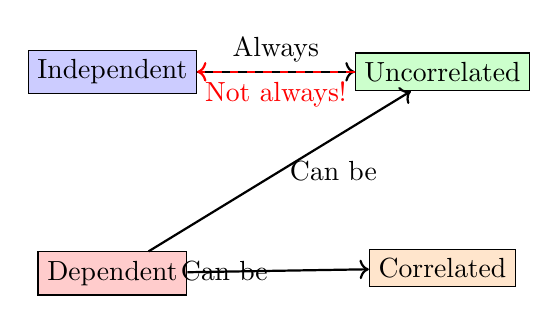
\begin{tikzpicture}[node distance=2cm, auto]
    % Nodes
    \node[draw, rectangle, fill=blue!20] (indep) {Independent};
    \node[draw, rectangle, fill=green!20, right=of indep] (uncorr) {Uncorrelated};
    \node[draw, rectangle, fill=orange!20, below=of uncorr] (corr) {Correlated};
    \node[draw, rectangle, fill=red!20, below=of indep] (dep) {Dependent};
    
    % Arrows
    \draw[->, thick] (indep) -- (uncorr) node[midway, above] {Always};
    \draw[->, thick, dashed, red] (uncorr) -- (indep) node[midway, below] {Not always!};
    \draw[->, thick] (dep) -- (corr) node[midway, left] {Can be};
    \draw[->, thick] (dep) -- (uncorr) node[midway, right] {Can be};
\end{tikzpicture}
\end{center}

% ============================================
% FINAL NOTES
% ============================================
\vfill

\begin{center}
\Large{\textbf{Good luck with your exam!}}

\vspace{1em}

\normalsize{Remember: Practice problems are the key to success.}

\vspace{0.5em}

\normalsize{Understanding > Memorization}
\end{center}

\end{document}
